\documentclass[12pt,a4paper]{article}
\usepackage[left=25mm,right=20mm,top=20mm,bottom=23mm]{geometry}
\usepackage{fontspec}
\setmainfont{NimbusRoman-Regular.otf}[BoldFont=NimbusRoman-Bold.otf,ItalicFont=NimbusRoman-Italic.otf,BoldItalicFont=NimbusRoman-BoldItalic.otf]
\setsansfont{DejaVu Sans}
\setmonofont{DejaVu Sans Mono}[Scale=0.78]
\usepackage{polyglossia}
\setdefaultlanguage{russian}
\setotherlanguage{english}
\newfontfamily\cyrillicfont[Script=Cyrillic,BoldFont=NimbusRoman-Bold.otf,ItalicFont=NimbusRoman-Italic.otf,BoldItalicFont=NimbusRoman-BoldItalic.otf]{NimbusRoman-Regular.otf}
\newfontfamily\cyrillicfontsf[Script=Cyrillic]{DejaVu Sans}
\newfontfamily\cyrillicfonttt[Script=Cyrillic,Scale=0.78]{DejaVu Sans Mono}
\usepackage{amsmath,amssymb,booktabs,array,tabularx,float,graphicx,enumitem,setspace,caption}
\usepackage[unicode,hidelinks]{hyperref}
\usepackage{xurl}
\hypersetup{pdftitle={Автоматический отбор признаков в рекомендательной системе},pdfauthor={Начаров Тимур Дмитриевич}}
\setstretch{1.10}
\setlength{\parindent}{1.25cm}
\setlength{\parskip}{2pt}
\setlist{itemsep=2pt,topsep=4pt}
\captionsetup{font=small,labelsep=colon}
\renewcommand{\arraystretch}{1.12}
\emergencystretch=4em
\sloppy
\widowpenalty=10000
\clubpenalty=10000
\displaywidowpenalty=10000
\newcommand{\code}[1]{\nolinkurl{#1}}
\begin{document}
\begin{titlepage}
\centering
\vspace*{22mm}
{\large ИССЛЕДОВАТЕЛЬСКАЯ РАБОТА\par}
\vspace{24mm}
{\LARGE\bfseries Автоматический отбор признаков\par}
\vspace{5mm}
{\Large в рекомендательной системе\par}
\vspace{7mm}
{\large Исследование реляционных и временных признаков\\на данных KION\par}
\vspace{30mm}
\begin{flushright}
Выполнил:\\[3mm]
Начаров Тимур Дмитриевич
\end{flushright}
\vfill
Москва, 2026
\end{titlepage}
\setcounter{page}{1}
\tableofcontents
\clearpage

\section{Цель работы}
Целью работы является исследование способов автоматического построения и
отбора признаков для рекомендательной системы, использующей градиентный
бустинг, а также определение влияния временных признаков на качество
ранжирования и вычислительные затраты.

Для достижения поставленной цели решаются следующие задачи:
\begin{enumerate}
\item Построить воспроизводимую двухэтапную систему рекомендаций и
содержательный набор ручных признаков.
\item Реализовать генерацию исторических агрегатов и сравнить отбор
по взаимной информации, условной взаимной информации и направленный поиск.
\item Исследовать полноту извлечения кандидатов при одинаковом размере списка.
\item Сравнить методы на общей тестовой выборке, сохраняя одинаковые
кандидаты, доступную историю и обучающие данные внутри каждого повтора.
\item Оценить устойчивость выбранных признаков и отдельно проверить
влияние коэффициентов временного затухания.
\item Проанализировать вычислительные затраты и ограничения полученных выводов.
\end{enumerate}

\section{Теоретические сведения}
\subsection{Двухэтапная рекомендательная система}
Для пользователя $u$ на момент времени $t$ сначала формируется множество
кандидатов $C_u(t)$, после чего модель вычисляет оценки $s(u,i,t)$ и
упорядочивает объекты $i\in C_u(t)$. В качестве результата выдаются первые
десять объектов списка. Первый этап ограничивает набор доступных ранкеру
объектов, поэтому качество извлечения кандидатов исследуется отдельно.

В работе применяются популярностные и жанровые источники, ItemKNN,
факторизация ALS и линейная модель EASE. ItemKNN использует связи между
объектами по совместным взаимодействиям пользователей. ALS приближает
матрицу implicit-взаимодействий произведением низкоранговых матриц.
EASE восстанавливает взаимодействия линейной моделью с регуляризацией
и нулевой диагональю матрицы весов. Списки нескольких источников объединяются
по reciprocal-rank fusion. В окончательном сравнении ранкером является
CatBoostRanker с функцией потерь YetiRank.

\subsection{Реляционные и временные признаки}
Признаки строятся по истории $H(t)=\{(u,i,\tau):\tau<t\}$.
Реляционный агрегат описывает связь пользователя с объектом через
совпадение жанров, страны, режиссёра или типа контента. Дополнительно
используются статистики пользователя и объекта.

Например, число совпадений в заданном интервале возраста событий имеет вид
\begin{equation}
x_{ui}^{(l,r)}(t)=\sum_{j\in H_u(t)}
\mathbf{1}\{l<t-\tau_j\le r\}\,
\mathbf{1}\{A(i)\cap A(j)\ne\varnothing\},
\end{equation}
где $A(i)$ — множество атрибутов объекта. В грамматику входят число
совпадений, их доля, давность последнего совпадения и число дней активности.
Используются накопительные окна, интервалы возраста и экспоненциальные ядра.

Автоматизация состоит в перечислении допустимых спецификаций и выборе
их подмножества. Семейства отношений и агрегатов задаются заранее;
поиск не выходит за пределы этой грамматики.

\subsection{Отбор по взаимной информации}
Для дискретизированного признака $X$ и целевой переменной $Y$ взаимная
информация определяется выражением
\begin{equation}
I(X;Y)=\sum_{x,y}p(x,y)\log\frac{p(x,y)}{p(x)p(y)}.
\end{equation}
Метод MI выбирает признаки с наибольшими значениями $I(X;Y)$.
В CMIM используется исторический контекст $C$: группы активности
пользователя, жанрового соответствия и популярности объекта.
Первый признак выбирается по $I(X;Y\mid C)$, а последующие — по оценке
\begin{equation}
q(X)=\min\left\{I(X;Y\mid C),\;\min_{Z\in S}I(X;Y\mid C,Z)\right\},
\end{equation}
где $S$ — уже выбранный набор. Это попарная эвристика уменьшения
избыточности; она не равна полной совместной условной информации.
Границы дискретизации определяются только на обучающих строках.
В ранкер передаются исходные числовые признаки.

В варианте CMIM + OOF в контекст дополнительно включается группа ранга
прогноза ручного baseline. Прогноз для каждой обучающей недели строится
моделью, обученной только на более ранних неделях. Сам OOF-score не
передаётся итоговому ранкеру: исследуется именно изменение отбора.

\subsection{Временное затухание}
Для исторического события $j$ с возрастом $a_j$ задаётся вес
\begin{equation}
w_{uij}=2^{-a_j/h_u}(1+\alpha R_{uj})(1+\beta S_{ij}),
\end{equation}
где $S_{ij}$ — сходство жанров по Жаккару, $R_{uj}$ — характеристика
регулярности жанровой истории, $h_u$ — период полураспада.
Регулярность учитывает разброс интервалов между днями активности и
сжимается при малом числе наблюдений.

Из весов формируются три входа ранкера:
\begin{equation}
\operatorname{affinity}=\frac{\sum_j w_{uij}S_{ij}}{\sum_jw_{uij}},\qquad
\operatorname{mass}=\log\left(1+\sum_jw_{uij}S_{ij}\right),\qquad
\operatorname{ESS}=\frac{(\sum_jw_{uij})^2}{\sum_jw_{uij}^2}.
\end{equation}
В контрольном варианте без затухания $w_{uij}=1$. Он позволяет отделить
эффект времени от эффекта добавления самих агрегатов сходства.

Общая зависимость периода полураспада от активности задаётся формулой
\begin{equation}
h_u=\operatorname{clip}\left[
h\left(\frac{g_u+1}{8}\right)^{\gamma n_u/(n_u+10)},\;0{,}25,\;180\right],
\end{equation}
где $n_u$ — длина истории, $g_u$ — медианный интервал между наблюдаемыми
днями активности. Параметры $h$ и $\gamma$ общие для пользователей.
Свободные индивидуальные коэффициенты не обучаются.

\subsection{Метрики качества}
Пусть $T_u$ — полное множество релевантных объектов пользователя
в следующей неделе, $r_{ui}$ — бинарная релевантность объекта на позиции $i$.
Полнота кандидатов и полнота рекомендаций определяются как
\begin{equation}
\operatorname{CandidateRecall}=\frac{1}{|U|}\sum_u
\frac{|C_u\cap T_u|}{|T_u|},\qquad
\operatorname{Recall@10}=\frac{1}{|U|}\sum_u
\frac{\sum_{i=1}^{10}r_{ui}}{|T_u|}.
\end{equation}
Основная метрика ранжирования:
\begin{equation}
\operatorname{NDCG@10}=\frac{1}{|U|}\sum_u
\frac{\sum_{i=1}^{10}r_{ui}/\log_2(i+1)}
{\sum_{i=1}^{\min(10,|T_u|)}1/\log_2(i+1)}.
\end{equation}
Дополнительно вычисляется MAP@10 с используемой в реализации нормировкой
\begin{equation}
\operatorname{AP@10}(u)=\frac{1}{\min(10,|T_u|)}
\sum_{i=1}^{10}P_u@i\,r_{ui},\qquad
\operatorname{MAP@10}=\frac{1}{|U|}\sum_u\operatorname{AP@10}(u).
\end{equation}
В знаменателях учитываются все будущие релевантные объекты, включая
отсутствующие в кандидатах и доступном каталоге. Пользователи без попаданий
не исключаются из оценки.

\section{Данные и параметры вычислительного эксперимента}
\subsection{Датасет и постановка задачи}
Используется русскоязычный вариант KION\footnote{Источник данных:
\url{https://github.com/irsafilo/KION_DATASET}.}: таблицы взаимодействий,
пользователей и объектов. В закреплённой версии содержится 5\,476\,251
строка взаимодействий 962\,179 пользователей с 15\,706 объектами.
Наблюдаемый период — 13 марта – 22 августа 2021 года.
Медианная длина истории равна двум объектам; у 73,54\% пользователей
наблюдается не более пяти объектов. Это характеристики всего датасета.
В общей тестовой когорте из 5000 warm-пользователей медиана числа
прошлых взаимодействий на срезе 16 августа равна 7; доля историй длиной
не более пяти составляет 44,42\%. Поэтому медиану всего датасета нельзя
непосредственно использовать как объяснение результатов на тестовой когорте.

На каждой дате среза требуется рекомендовать объекты следующей недели.
История ограничивается условием $\tau<t$, включая исключение дня среза.
Каталог формируется из объектов с прошлым взаимодействием, наблюдавшиеся
ранее пары исключаются из кандидатов. Будущие положительные объекты
искусственно в список не добавляются.

KION содержит последнюю дату взаимодействия пары пользователь–объект,
а не полный журнал просмотров. Журнал показов отсутствует. Поэтому
нулевая метка означает отсутствие наблюдаемого взаимодействия в горизонте,
но не подтверждённый отказ после показа. Оцениваются пользователи,
имеющие прошлую историю и хотя бы одно будущее событие.

\subsection{Обучающая, валидационная и тестовая выборки}
Для общего сравнения используется единое временное разбиение,
приведённое в таблице~\ref{tab:split}. Внутри каждого повтора методы
получают одинаковые обучающие строки; на тесте для всех повторов
фиксируются одни пользователи и кандидаты.
\begin{table}[H]
\centering
\small
\caption{Временная схема общего сравнения}\label{tab:split}
\begin{tabular}{llr}\toprule
Назначение & Даты срезов / горизонт & Пользователей \\ \midrule
Обучение & 12, 19, 26 июля; 2 августа & 2000 на срез \\
Валидация & 9–15 августа & 5000 \\
Тест & 16–22 августа & 5000 \\
\bottomrule
\end{tabular}
\end{table}
Для построения глобальных агрегатов и retrieval используется вся
доступная прошлая история, а не только выбранные query-пользователи.
Обучение ранкера ограничивается 2000 пользователями на каждом из четырёх
срезов. Обучающие когорты выбираются из фиксированного пула 5000 пользователей.
Сохраняются все найденные положительные кандидаты и не более 48
случайных нулевых кандидатов на запрос.

Применяются три значения seed: 17, 42 и 73. Они изменяют обучающие
когорты, sampling нулей и случайность обучения. Валидационные и тестовые
пользователи общие для методов и seeds. Все решения сохраняются до
начала тестового применения моделей. После выбора обучение на validation
не проводится: итоговые модели используют одинаковые четыре train-среза.

Августовские периоды уже рассматривались на предыдущих этапах исследования.
Следовательно, общее разбиение обеспечивает сопоставимость вариантов,
но не является независимым, ранее не использованным контрольным периодом.

\subsection{Ручной baseline и автоматический поиск}
Ручной baseline содержит 56 признаков: характеристики пользователя и
объекта, активность и давность, популярности за разные интервалы,
соответствие жанрам, реляционные агрегаты и признаки retrieval.
После удаления констант и дубликатов доступны 131 дополнительные
спецификации. Полный вариант содержит 187 входов, а компактные
MI/CMIM-наборы — по 68, то есть baseline и 12 выбранных добавлений.

Случайный поиск сравнивает восемь уникальных наборов по 12 признаков.
Направленный поиск начинает с MI и CMIM, затем изменяет лучший по
validation набор, заменяя до трёх признаков. Он также рассматривает восемь
уникальных наборов. Граница числа проб одинакова, но направленный метод
дополнительно затрачивает ресурсы на оценку информативности.

MI, CMIM и CMIM + OOF используют одинаковые sampled строки последних трёх
train-срезов. Первый срез входит в финальное обучение и используется как
предыстория для OOF, но не для отбора. Группы без положительных кандидатов
исключаются из ranking loss; при оценке и расчёте информативности они
сохраняются. Параметры ранкера фиксированы для всех вариантов.
\begin{table}[H]
\centering
\small
\caption{Общие параметры ранкера и оценки}\label{tab:params}
\begin{tabular}{ll}\toprule
Параметр & Значение \\ \midrule
Число деревьев & 200 \\
Глубина & 4 \\
Скорость обучения & 0,07 \\
L2-регуляризация & 5 \\
Функция потерь & \code{YetiRank:permutations=1} \\
Обработка категорий & One-hot \\
Бюджет кандидатов & 100 \\
Число bootstrap-повторов & 2000 \\
\bottomrule
\end{tabular}
\end{table}
\subsection{Программная реализация и оценка неопределённости}
Расчёты выполнены на Python с использованием NumPy, pandas, SciPy,
CatBoost и implicit. В общем эксперименте использованы CatBoost 1.2.10,
implicit 0.7.2 и шесть CPU-потоков. Сохраняются конфигурации, выбранные
признаки, модели, общие кандидаты, top-10 и метрики каждого пользователя.

Для парной разности NDCG пользователи повторно выбираются с возвращением;
для каждого seed строится 95\%-й percentile bootstrap-интервал по 2000
повторам. Он условен на уже обученных моделях. Среднее и стандартное
отклонение по трём seeds характеризуют наблюдаемый разброс, но не дают
полного распределения качества процесса обучения. Среднее качество
отдельных ранкеров не является качеством ансамбля их scores.

\section{Исследование извлечения кандидатов}
\subsection{Постановка эксперимента}
Сравниваются популярностно-жанровый источник, ItemKNN, ALS, EASE и
их объединения. Каждый список дополняется прошлой популярностью до
100 объектов при достаточном каталоге; известная история исключается.
Когорты и truth внутри каждой недели одинаковы. Параметры источников
и состав объединения выбираются на предшествующей валидационной неделе.

В ALS проверены 32/64 латентных факторов, 15 итераций, регуляризация 0,1
и confidence-параметр 20. EASE ограничен 4000 наиболее популярными
в прошлом объектами; проверены коэффициенты регуляризации 500 и 1000.
В таблице~\ref{tab:retrieval} приведена полнота кандидатов отдельной серии.
Её когорты отличаются от окончательного общего теста.
\begin{table}[H]
\centering
\small
\caption{Candidate recall при бюджете 100}\label{tab:retrieval}
\begin{tabular}{lrr}\toprule
Источник & 9 августа & 16 августа \\ \midrule
Популярность и жанры & 0,403174 & 0,419775 \\
ItemKNN & 0,427489 & 0,422258 \\
ALS & 0,357865 & 0,355216 \\
EASE & 0,437251 & 0,437694 \\
Популярность/жанры + KNN & 0,442503 & 0,451291 \\
Популярность/жанры + KNN + EASE & 0,457963 & 0,464137 \\
Объединение всех источников & 0,462133 & 0,460651 \\
\bottomrule
\end{tabular}
\end{table}
\subsection{Результаты выбора источников}
В обоих случаях validation выбрала объединение популярности/жанров,
ItemKNN и EASE. Добавление EASE к популярности/жанрам и KNN повысило
полноту на 1,55 и 1,28 процентного пункта соответственно. Добавление всех
источников не гарантирует улучшения: при фиксированной длине новые
кандидаты могут вытеснять более полезные.

ALS в проверенной небольшой сетке оказался слабее остальных одиночных
источников. Это относится к конкретным параметрам и бинарному представлению
истории. Полный каталог для EASE не исследовался.

В окончательном общем сравнении зафиксировано объединение с EASE.
На его 5000 тестовых пользователях candidate recall равен 0,471633 для
всех методов. Новая величина относится к общей когорте и не подставляется
в таблицу отдельного retrieval-эксперимента. Оставшиеся потери полноты
ограничивают доступ ранкера к будущим положительным объектам.

\section{Результаты сравнения на общем тесте}
\subsection{Качество ранжирования}
Таблица~\ref{tab:quality} содержит средние метрики трёх отдельных моделей
для каждого метода. Число входов включает ручной baseline.
Параметры затухания и наборы признаков выбирались по validation,
а не по результатам этой таблицы.
\begin{table}[H]
\centering
\small
\caption{Качество на общем тесте 16–22 августа}\label{tab:quality}
\begin{tabular}{lrrrrr}\toprule
Метод & Входы & NDCG@10 & $s_{\rm seeds}$ & MAP@10 & Recall@10 \\ \midrule
Ручной baseline & 56 & 0,154842 & 0,000487 & 0,102630 & 0,237578 \\
Весь банк & 187 & 0,156234 & 0,000416 & 0,104159 & 0,237855 \\
MI & 68 & 0,156136 & 0,000277 & 0,104222 & 0,237601 \\
CMIM & 68 & 0,156365 & 0,000679 & 0,104012 & 0,238462 \\
CMIM + OOF & 68 & 0,156265 & 0,001031 & 0,104042 & 0,238380 \\
Случайный поиск & 68 & 0,154898 & 0,000806 & 0,103080 & 0,236401 \\
Направленный поиск & 68 & 0,156701 & 0,000567 & 0,104590 & 0,238267 \\
Без затухания & 59 & 0,155558 & 0,000848 & 0,103467 & 0,238007 \\
Постоянный h & 59 & 0,155611 & 0,000917 & 0,103850 & 0,237015 \\
Подбор $\alpha$ & 59 & 0,155490 & 0,000969 & 0,103752 & 0,236870 \\
Подбор $\beta$ & 59 & 0,155265 & 0,000954 & 0,103490 & 0,236885 \\
Адаптивный h & 59 & 0,156189 & 0,001427 & 0,104295 & 0,237989 \\
Несколько ядер & 71 & 0,156406 & 0,000340 & 0,104369 & 0,238328 \\
Поиск + несколько ядер & 83 & 0,156363 & 0,000090 & 0,103925 & 0,239045 \\
CMIM + затухание & 71 & 0,156904 & 0,000983 & 0,104675 & 0,238661 \\
\bottomrule
\end{tabular}
\end{table}
Ручной baseline достигает NDCG@10 = 0,154842. Направленный поиск
даёт 0,156701, что соответствует абсолютному приросту 0,001859
(около 1,20\% относительно baseline). CMIM достигает 0,156365,
а использование всего банка — 0,156234.

Наибольшее среднее среди проверенных вариантов получено для CMIM
с затуханием: 0,156904. Это описательная характеристика общего теста;
она не используется для назначения нового итогового метода.
По validation были выбраны весь банк для seed 17 и направленный поиск
для seeds 42 и 73.

\subsection{Парные разности и разброс по повторам}
Основным заранее заданным сравнением является направленный поиск
относительно ручного baseline. Для отделения роли направленного поиска
дополнительно рассматривается его разность со случайным поиском.
\begin{table}[H]
\centering
\small
\caption{Парные bootstrap-интервалы}\label{tab:paired}
\begin{tabular}{llrl}\toprule
Seed & Сравнение & $\Delta$ NDCG & 95\%-й интервал \\ \midrule
17 & Поиск – baseline & +0,001579 & [+0,000003; +0,003114] \\
17 & Поиск – случайный & +0,001966 & [+0,000450; +0,003569] \\
42 & Поиск – baseline & +0,001913 & [+0,000610; +0,003296] \\
42 & Поиск – случайный & +0,002641 & [+0,001208; +0,004054] \\
73 & Поиск – baseline & +0,002086 & [+0,000470; +0,003734] \\
73 & Поиск – случайный & +0,000803 & [-0,000605; +0,002199] \\
\bottomrule
\end{tabular}
\end{table}
Относительно baseline разность положительна во всех трёх seeds,
и все три условных интервала лежат выше нуля. Для seed 17 нижняя граница
очень близка к нулю. Относительно случайного поиска положительны все три
разности, однако только два интервала не пересекают ноль.
Поправка на множественные сравнения не применялась.

\begin{figure}[H]
\centering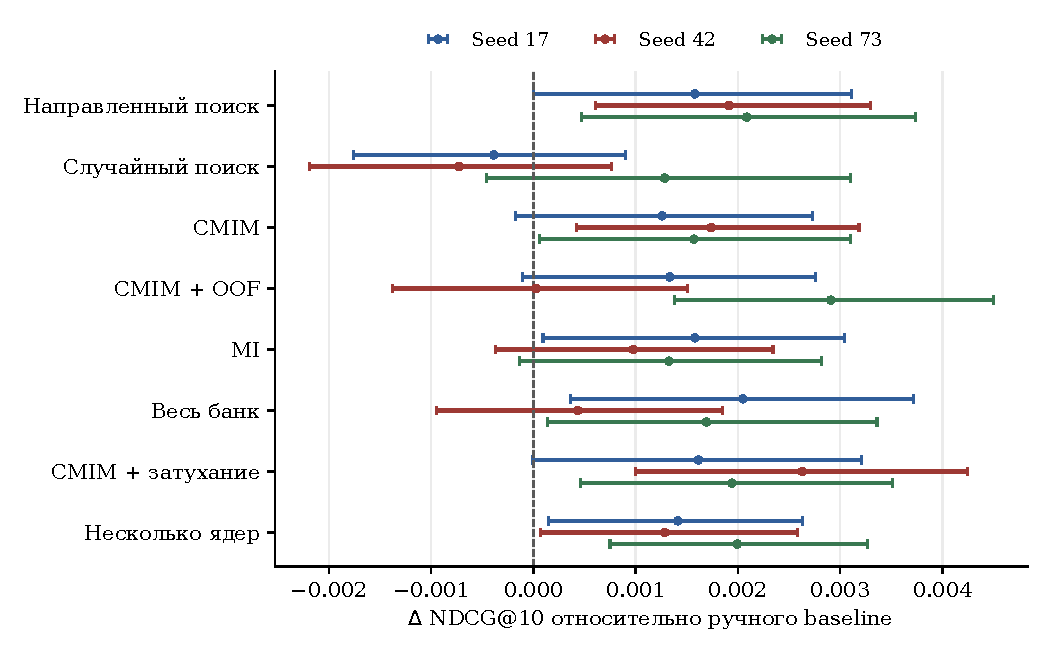
\includegraphics[width=\linewidth]{paired_ndcg.pdf}
\caption{Разности NDCG@10 относительно ручного baseline и 95\%-е
парные user-bootstrap-интервалы. Каждый цвет соответствует отдельному seed.}
\label{fig:paired}
\end{figure}

MI, CMIM, весь банк, направленный поиск и его сочетание с несколькими ядрами имеют
положительное среднее улучшение во всех трёх повторах. При этом рост NDCG
не означает аналогичного роста Recall: например, случайный поиск почти
не меняет NDCG и уменьшает средний Recall. Разные метрики отражают
разные свойства порядка объектов.

\section{Устойчивость автоматического отбора}
\subsection{Схема дополнительного исследования}
Устойчивость исследуется отдельно на июльских валидационных неделях
12, 19 и 26 июля. Для каждой даты используются четыре предыдущие
train-недели, размеры когорт 700/2000 и seeds 17/42/73.
Retrieval зафиксирован, бюджет равен 100. Меньшая train-когорта внутри
seed вложена в большую; общий feature-пул составляет 8000 пользователей
на срез и не является размером обучения ранкера.

Совпадение двух выбранных наборов оценивается коэффициентом Жаккара
\begin{equation}
J(S_1,S_2)=\frac{|S_1\cap S_2|}{|S_1\cup S_2|}.
\end{equation}
Отдельно сравниваются точные спецификации и временные окна без учёта
отношения и агрегата. Поэтому совпадение окон и совпадение признаков
являются разными характеристиками.

\subsection{Влияние размера обучающей когорты}
\begin{table}[H]
\centering
\small
\caption{Средний Jaccard между seeds в июльской серии}\label{tab:stability}
\begin{tabular}{rlrr}\toprule
Train-пользователи & Метод & Признаки & Окна \\ \midrule
700 & MI & 0,880 & 0,880 \\
700 & CMIM & 0,570 & 0,768 \\
700 & CMIM + OOF & 0,437 & 0,674 \\
2000 & MI & 0,932 & 0,932 \\
2000 & CMIM & 0,584 & 0,751 \\
2000 & CMIM + OOF & 0,691 & 0,822 \\
\bottomrule
\end{tabular}
\end{table}
\begin{figure}[H]
\centering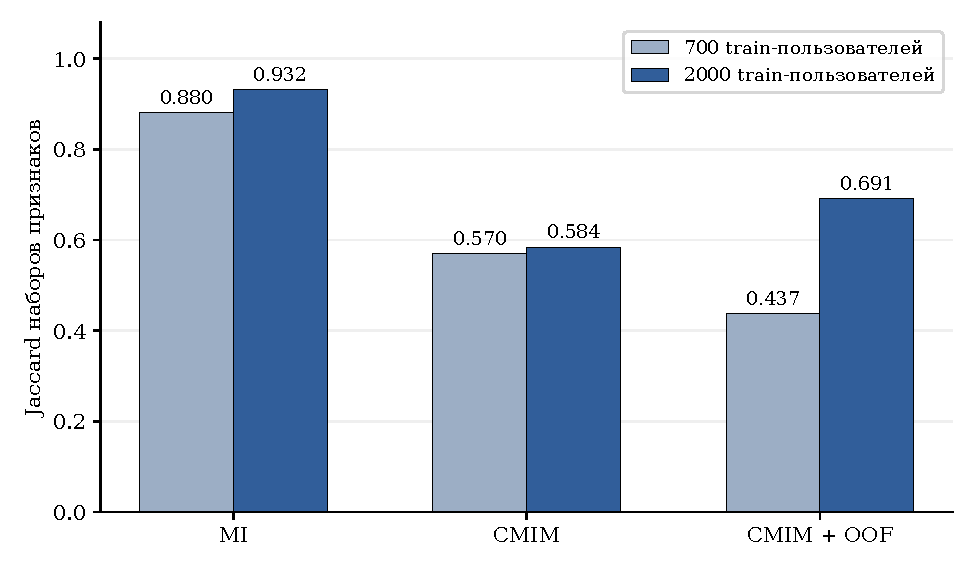
\includegraphics[width=.90\linewidth]{selection_stability.pdf}
\caption{Устойчивость точных наборов признаков при изменении размера train-когорты.}
\label{fig:stability}
\end{figure}

MI даёт наиболее устойчивые точные наборы. У CMIM + OOF Jaccard
признаков увеличивается с 0,437 до 0,691, а окон — с 0,674 до 0,822.
Увеличение размера сопровождается большим пересечением когорт,
выбранных из фиксированного пула; поэтому весь эффект нельзя приписать
только улучшению оценки информативности.

При сравнении временных фолдов для 2000 пользователей Jaccard точных
наборов равен 0,949 для MI, 0,640 для CMIM и 0,643 для CMIM + OOF.
Меньшее совпадение состава не обязательно означает нестабильное качество:
коррелированные временные агрегаты могут заменять друг друга.

\subsection{Влияние OOF-контроля baseline}
В июльской серии дополнительный контроль baseline выигрывает у CMIM
в 7 из 18 сравнений. При 2000 пользователях его средняя разность NDCG
к CMIM составляет примерно $-0,000123$. Состав отбора меняется:
снижается доля item-признаков, но это не обеспечивает устойчивого роста
качества ранжирования.

На общем августовском тесте средняя разность CMIM + OOF к CMIM равна
$-0,000100$. Два seed дают положительную разность, один — отрицательную;
по одному интервалу целиком выше и ниже нуля. Таким образом, устойчивой
пользы дополнительного conditioning не установлено. Возможные причины —
разреженность условных страт и расхождение между построчной
информативностью и ranking-целью.

\section{Исследование временных признаков}
\subsection{Разделение эффектов и выбор периода полураспада}
При фиксированном жанровом сходстве сначала сравниваются только
$h\in\{1,3,7,14,30\}$ при $\alpha=\beta=\gamma=0$.
Затем при выбранном $h$ независимо проверяются $\alpha\in\{0{,}5,1,2\}$,
$\beta\in\{0{,}5,1,2\}$ и $\gamma\in\{0{,}5,1\}$.
Каждая ветка содержит нулевой вариант, поэтому validation может
отказаться от дополнительного множителя. Совместный перебор всех
сочетаний не проводится.

В отдельной ранней калибровке на 5–11 июля выбирался $h=1$ день.
В общем августовском протоколе validation выбирает 14/7/7 дней.
Эти результаты относятся к разным периодам и обучающим данным:
универсальный оптимальный half-life из них не следует.
\begin{table}[H]
\centering
\small
\caption{Параметры, выбранные на общей validation в независимых ветках}\label{tab:decaychoices}
\begin{tabular}{rrrrr}\toprule
Seed & $h$, дней & $\alpha$ & $\beta$ & $\gamma$ \\ \midrule
17 & 14 & 0 & 0 & 0 \\
42 & 7 & 2 & 0 & 0,5 \\
73 & 7 & 2 & 0,5 & 1,0 \\
\bottomrule
\end{tabular}
\end{table}
Значения $\alpha$, $\beta$, $\gamma$ в таблице~\ref{tab:decaychoices}
относятся к разным моделям, а не к одному совместному kernel.
Для seed 17 все дополнительные множители отклонены по validation.

\subsection{Роль временного затухания}
На общем тесте вариант без затухания имеет средний NDCG 0,155558,
а constant decay — 0,155611. Средняя разность составляет всего
0,000052 и положительна лишь в одном из трёх seeds.
Следовательно, улучшение относительно ручного baseline нельзя целиком
объяснить временем: часть информации содержится в самих агрегатах сходства.

Выбранные по validation $\alpha$ и $\beta$ не улучшают среднее качество
относительно constant decay. Адаптивный $h$ даёт более высокое среднее
NDCG 0,156189, но разброс по seeds велик: стандартное отклонение 0,001427.
Формула меняет как различия между пользователями, так и средний масштаб
памяти. Без контроля с согласованным общим масштабом её эффект нельзя
приписать одной персонализации.

В раннем июльском анализе у 86–87\% пользователей с 1–5 событиями
регулярность $R$ равна нулю, и $\alpha$ не изменяет их признаки.
Это ограничивает чувствительность коротких историй к данному механизму.

\subsection{Несколько временных ядер и комбинированные признаки}
Многомасштабный вариант объединяет три агрегата для каждого из пяти
half-life, добавляя 15 входов. Это фиксированная конкатенация,
а не обучаемая смесь. Его средний NDCG равен 0,156406.
Совмещение с направленным поиском даёт 0,156363 и не улучшает
результат отдельного направленного поиска.

CMIM с выбранным constant decay достигает 0,156904 и имеет положительную
разность к baseline во всех seeds. Этот локальный результат показывает
полезность конкретного сочетания признаков, но не доказывает отдельный
эффект каждого компонента или пользу индивидуальных свободных параметров.

\section{Вычислительные затраты и ограничения}
\subsection{Стоимость обучения и поиска}
В таблице~\ref{tab:cost} приведены средние времена на CPU для выбранных
моделей общего сравнения. Время применения включает загрузку модели,
получение предсказаний, расчёт метрик и сохранение результатов;
оно не является чистой задержкой обслуживания запроса.
\begin{table}[H]
\centering
\small
\caption{Средние времена выбранных моделей на общем протоколе}\label{tab:cost}
\begin{tabular}{lrr}\toprule
Модель & Обучение, с & Применение и оценка, с \\ \midrule
Ручной baseline & 9,69 & 1,51 \\
Весь банк & 14,18 & 1,92 \\
MI & 9,73 & 1,55 \\
CMIM & 9,81 & 1,50 \\
CMIM + OOF & 9,90 & 1,45 \\
Направленный поиск & 9,88 & 1,41 \\
CMIM + затухание & 10,51 & 1,42 \\
\bottomrule
\end{tabular}
\end{table}
На каждый seed приходится 36 уникальных validation-fit,
суммарно около 357–371 с чистого обучения моделей. Три forward OOF-fit
добавляют около 15 с на seed. Сам CMIM требует примерно 2,3–2,4 с,
а CMIM + OOF — 2,4–2,6 с без учёта стоимости OOF-моделей.
В эти величины не включены загрузка исходных данных, построение
retrieval, генерация всех признаков и затраты оценки trial-моделей.

Сокращение 187 входов до 68 уменьшает размер набора для ранкера,
но полный банк сначала вычисляется для поиска. Следовательно,
уменьшение числа входов не означает автоматически такое же ускорение
всего эксперимента. Для применения уже найденного набора достаточно
вычислять только выбранные агрегаты.

У направленного поиска 68 входов вместо 187 у полного банка: сокращение
составляет 63,6\%. Наблюдаемое среднее NDCG равно соответственно
0,156701 и 0,156234. Это близкие значения на данном тесте, но специальная
проверка эквивалентности или не меньшей эффективности с заранее заданным
допуском не проводилась. Поэтому статистическая эквивалентность не утверждается.
Число исходных ручных входов равно 56: переход 187 к 68 сравнивает
компактный вариант с полным банком, а не с ручным baseline.

Ускорение чистого инференса и снижение переобучения отдельно не установлены.
При фиксированных числе деревьев и глубине стоимость прохода по деревьям
не обязана уменьшаться пропорционально числу входных колонок.
Снижение стоимости производства признаков после отбора является
обоснованным направлением оптимизации, а не измеренным ускорением всего сервиса.

\subsection{Ограничения данных и статистической оценки}
Главное ограничение источника связано с последней датой пары:
для раннего среза неизвестны предыдущие просмотры, если финальная дата
взаимодействия находится позже него. Статические метаданные не содержат
журнала исторических изменений. Модель описывает доступный экспорт,
а не полностью восстановленное состояние сервиса в прошлом.

Результаты условны на warm-пользователях с будущей активностью.
Отсутствие impression log не позволяет трактовать нули как
экспозиционно подтверждённые негативы или ranking-score как вероятность клика.
Качество холодного старта и аудитории без будущих событий здесь не оценено.

Общий августовский test уже использовался в предыдущих исследованиях.
Положительные результаты характеризуют текущую постановку и требуют
проверки на новом периоде либо другом датасете для независимого подтверждения.
Три seeds используют общую тестовую когорту и не являются независимыми
выборками пользователей. Июльские временные фолды также перекрываются.

Условные bootstrap-интервалы не учитывают все шаги поиска гипотез,
неопределённость всего процесса обучения и множественные сравнения.
Проверен ограниченный набор параметров. Для EASE использован словарь
4000 объектов; производительность полного каталога и промышленная
масштабируемость не установлены.

\subsection{Воспроизведение эксперимента}
К отчёту приложен каталог \code{kion_common_test} с кодом, конфигурациями,
зафиксированными версиями зависимостей и сохранёнными результатами.
Из его корня выполняются следующие команды:
\begin{small}\begin{verbatim}
python -m pip install -e '.[dev,retrieval]'
python scripts/download_data.py
OPENBLAS_NUM_THREADS=1 OMP_NUM_THREADS=6 PYTHONPATH=src \
 python -m kion_recsys.common_test --config configs/common_test.json
PYTHONPATH=src python scripts/verify_common_test.py
python -m pytest -q
\end{verbatim}\end{small}
Команды с переменными окружения приведены для Bash. На других системах
переменные задаются соответствующим способом. Исходный архив KION
загружается из закреплённого commit с проверкой SHA-256. Ограничения
обучения, seeds, даты, кандидаты и сетки задаются в
\code{configs/common_test.json}.

Сохранённые результаты можно проверить без нового обучения. Для полного
повторного расчёта с нуля в копии конфигурации задаётся другой
\code{output_dir}. Прежний каталог не удаляется: обычный повтор команды
использует его checkpoints. Данные и большие feature-кэши в поставку
не включаются. Численные результаты могут не совпадать побитово при
изменении среды, поэтому приложены версии библиотек и параметры расчёта.

\section{Заключение}
В работе построена двухэтапная рекомендательная система с общим
градиентным бустингом. Предложенный метод является автоматизированным
отбором из заданной экспертом грамматики, а не генеративным построением
признаков. Автоматически перечисляются и отбираются предусмотренные
грамматикой агрегаты; новые отношения и операции вне неё не открываются.

Добавление EASE к популярностно-жанровому и ItemKNN-источникам повысило
полноту кандидатов при одинаковом бюджете. В общем сравнении все методы
получили одинаковые 100 кандидатов и тестовую когорту из 5000 пользователей.

Основной практический результат — компактный набор из 68 входов вместо
187 у полного банка, то есть на 63,6\% меньше, при близком наблюдаемом
качестве: NDCG@10 = 0,156701 против 0,156234. Это описательное сравнение,
а не доказанная статистическая эквивалентность. Относительно ручного
baseline из 56 входов также получен небольшой локальный прирост
с 0,154842 до 0,156701. Он не скрывается, но не рассматривается как
доказательство общего превосходства метода на новых данных.

Отбор по MI показал наибольшую устойчивость точных наборов.
Дополнительный OOF-контроль изменяет состав CMIM-отбора, но устойчивого
прироста качества не даёт. Само временное затухание почти не отличается
от агрегатов без времени в среднем по общему тесту. Усложнение временной
модели не обеспечивает гарантированного улучшения. В пределах проверенных
параметров не получено устойчивого свидетельства полезности всех
добавочных множителей. Это отрицательный результат конкретного эксперимента,
а не строгое доказательство бесполезности сложных временных моделей.
Короткие истории являются возможным ограничивающим фактором, однако их
причинная роль отдельно не проверялась.

Сокращение числа входов не доказывает уменьшение переобучения или
ускорение чистого инференса. Подтверждены компактность набора и конкретные
измерения затрат; потенциальная экономия при производстве выбранных
агрегатов требует отдельной оценки. Для развития метода целесообразно
исследовать расширение грамматики и согласование цели отбора с
ranking-метрикой. Независимая проверка на новом периоде нужна как для
положительных, так и для отрицательных выводов.

\end{document}
